% !TEX TS-program = xelatex
% !TEX encoding = UTF-8 Unicode
% !Mode:: "TeX:UTF-8"

\documentclass{resume}
\usepackage{graphicx}
\usepackage{tabu}
\usepackage{tabularx}
\usepackage{multirow}
\usepackage{progressbar}
\usepackage{zh_CN-Adobefonts_external} % Simplified Chinese Support using external fonts (./fonts/zh_CN-Adobe/)
\usepackage{tikz}
% \usepackage{NotoSansSC_external}
% \usepackage{NotoSerifCJKsc_external}
% \usepackage{zh_CN-Adobefonts_internal} % Simplified Chinese Support using system fonts
\usepackage{linespacing_fix} % disable extra space before next section
\usepackage{cite}

\newcommand{\hlink}[1]{\href{#1}{#1}}

\begin{document}
\pagenumbering{gobble} % suppress displaying page number

\medskip\noindent
\begin{minipage}{0.7\textwidth}
  \Large{
    \begin{tabu}  { l }
      \scshape{彭 \quad  程} \\
      \email{pengcheng@live.ca} \\
      \phone{(+86) 13070157185} \\
    \end{tabu}
  }
\end{minipage}
\begin{minipage}{0.3\textwidth}
  \raggedleft
  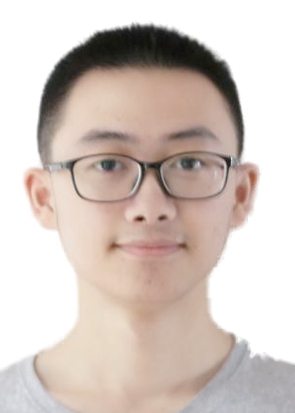
\includegraphics[height=30mm]{me}
\end{minipage}

\section{  教育背景}
\datedsubsection{\textbf{北京航空航天大学}, 北京}{2017 -- 至今}
\textit{在读硕士研究生}\quad {计算机学院} \quad{研究生专业学位硕士研究生考试总成绩第一录取 , 2020年1月毕业}
\datedsubsection{\textbf{北京航空航天大学}, 北京}{2013 -- 2017}
\textit{学士}\quad  {电子信息工程学院}\quad { 北斗实验班}

\section{ 实习/项目经历}

\datedsubsection{\textbf{大规模图像的分级快速检索}}{2017年12月 -- 至今}
\role{CNN 深度哈希}{研究生课题}
%\begin{onehalfspacing}
\begin{itemize}[topsep = 0 pt, partopsep = 0pt]
  \item 多级检索的快速深度哈希索引算法
  \item 百万量级图像库,百毫秒级相应,显著快于现有算法
  \item 实验与论文进行中
\end{itemize}
%\end{onehalfspacing}


\datedsubsection{\textbf{某部队遥感影像检测项目}}{2018年5月 -- 2019年1月}
\role{Mask R-CNN}{实验室项目}
%\begin{onehalfspacing}
\begin{itemize}[topsep = 0 pt, partopsep = 0pt]
  \item Mask R-CNN 遥感影像对地面建筑物的检测
  \item 不同时相遥感影像的变化检测
\end{itemize}
%\end{onehalfspacing}

\datedsubsection{\textbf{旷视科技数据平台建设}}{2017年7月 -- 2018年2月}
\role{Spark,Storm}{旷视CSG数据平台}
\begin{itemize}[topsep = 0 pt, partopsep = 0pt]
  \item Spark、Hive数据处理,协助数据分析师统计数据,识别可疑用户
  \item Storm 实时流处理,消费Kafka数据,实现实时报表统计
  \item Airflow 任务调度,自动化周期性任务
\end{itemize}

\datedsubsection{\textbf{基于虚拟现实技术的医学影像重建与交互系统}}{2016年6月 -- 2017年6月}
\role{Unity3D}{本科毕设,北航电子实验中心}
%\begin{onehalfspacing}
\begin{itemize}[topsep = 0 pt, partopsep = 0pt]
  \item CT、MRI等医疗影像的三维重建
  \item HTC Vive虚拟显示设备的显示与交互
  \item 可使用VR设备对三维人体模型切片,观察内部结构,辅助诊断与教学
\end{itemize}
%\end{onehalfspacing}

\section{技能}
% increase linespacing [parsep=0.5ex]
\begin{itemize}[parsep=0.5ex]
  \item 编程语言:常用 C/C++、Python,了解 Java、Scala、Golang
  \item 工具: Linux、Git、Docker
\end{itemize}

\section{获奖情况}
\datedline{\textit{国家励志奖学金}}{2014 年 8 月}
\datedline{\textit{北京航空航天大学新生奖学金}}{2017 年 8 月}

\section{ 其他}
% increase linespacing [parsep=0.5ex]
\begin{itemize}[parsep=0.5ex]
  \item  英语 - 熟练(CET-6 530)
  \item  无线电台呼号 BI1GPX
\end{itemize}

\end{document}
